% Options for packages loaded elsewhere
\PassOptionsToPackage{unicode}{hyperref}
\PassOptionsToPackage{hyphens}{url}
\PassOptionsToPackage{dvipsnames,svgnames,x11names}{xcolor}
\documentclass[
  11pt,
]{article}
\usepackage{xcolor}
\usepackage[margin=2.5cm]{geometry}
\usepackage{amsmath,amssymb}
\setcounter{secnumdepth}{-\maxdimen} % remove section numbering
\usepackage{iftex}
\ifPDFTeX
  \usepackage[T1]{fontenc}
  \usepackage[utf8]{inputenc}
  \usepackage{textcomp} % provide euro and other symbols
\else % if luatex or xetex
  \usepackage{unicode-math} % this also loads fontspec
  \defaultfontfeatures{Scale=MatchLowercase}
  \defaultfontfeatures[\rmfamily]{Ligatures=TeX,Scale=1}
\fi
\usepackage[]{charter}
\ifPDFTeX\else
  % xetex/luatex font selection
\fi
% Use upquote if available, for straight quotes in verbatim environments
\IfFileExists{upquote.sty}{\usepackage{upquote}}{}
\IfFileExists{microtype.sty}{% use microtype if available
  \usepackage[]{microtype}
  \UseMicrotypeSet[protrusion]{basicmath} % disable protrusion for tt fonts
}{}
\makeatletter
\@ifundefined{KOMAClassName}{% if non-KOMA class
  \IfFileExists{parskip.sty}{%
    \usepackage{parskip}
  }{% else
    \setlength{\parindent}{0pt}
    \setlength{\parskip}{6pt plus 2pt minus 1pt}}
}{% if KOMA class
  \KOMAoptions{parskip=half}}
\makeatother
\usepackage{graphicx}
\makeatletter
\newsavebox\pandoc@box
\newcommand*\pandocbounded[1]{% scales image to fit in text height/width
  \sbox\pandoc@box{#1}%
  \Gscale@div\@tempa{\textheight}{\dimexpr\ht\pandoc@box+\dp\pandoc@box\relax}%
  \Gscale@div\@tempb{\linewidth}{\wd\pandoc@box}%
  \ifdim\@tempb\p@<\@tempa\p@\let\@tempa\@tempb\fi% select the smaller of both
  \ifdim\@tempa\p@<\p@\scalebox{\@tempa}{\usebox\pandoc@box}%
  \else\usebox{\pandoc@box}%
  \fi%
}
% Set default figure placement to htbp
\def\fps@figure{htbp}
\makeatother
\setlength{\emergencystretch}{3em} % prevent overfull lines
\providecommand{\tightlist}{%
  \setlength{\itemsep}{0pt}\setlength{\parskip}{0pt}}
% ==========================================================================
%  IA na Sociedade — cabeçalho LaTeX (pdflatex)
%  Programa CiberExt 26-29 · FEELT38103
%  Adaptado de "AI in Society" (Universidade de Helsinque / Una Europa)
%  Licença: CC BY-NC-SA 4.0
% --------------------------------------------------------------------------
%  Espelha a identidade do ia-style.css: papel quente, tinta ardósia e a
%  faixa tricolor dos três eixos do curso (conceitos / aplicações / riscos).
% ==========================================================================

% ---------- Fontes ----------
% A serifada vem do build.sh, que passa  -V fontfamily=charter  ao pandoc.
% Aqui só acrescentamos a sem-serifa; ambas com fallback, porque nem toda
% instalação de LaTeX traz os mesmos pacotes.
\IfFileExists{helvet.sty}{\usepackage[scaled=0.90]{helvet}}{}
\usepackage{textcomp}
\IfFileExists{microtype.sty}{\usepackage{microtype}}{}

% ---------- Pacotes de layout ----------
\usepackage{xcolor}
\usepackage{tcolorbox}
\tcbuselibrary{skins,breakable}
\usepackage{titlesec}
\usepackage{fancyhdr}
\usepackage{enumitem}
\usepackage{amssymb}
\usepackage{booktabs}
\usepackage{array}
\usepackage{colortbl}
\usepackage{ragged2e}
\usepackage{fvextra}
\usepackage{newunicodechar}

% ---------- Caracteres Unicode que o pdflatex não conhece ----------
\newunicodechar{✓}{{\color{iaAplic}\checkmark}}
\newunicodechar{✅}{{\color{iaAplic}\checkmark}}
\newunicodechar{→}{\ensuremath{\rightarrow}}
\newunicodechar{←}{\ensuremath{\leftarrow}}
\newunicodechar{↔}{\ensuremath{\leftrightarrow}}
\newunicodechar{–}{--}
\newunicodechar{—}{---}
\newunicodechar{€}{\texteuro}
\newunicodechar{£}{\textsterling}
\newunicodechar{×}{\ensuremath{\times}}
\newunicodechar{≈}{\ensuremath{\approx}}
\newunicodechar{≥}{\ensuremath{\geq}}
\newunicodechar{≤}{\ensuremath{\leq}}
\newunicodechar{•}{\textbullet}
\newunicodechar{″}{''}
\newunicodechar{′}{'}

% ==========================================================================
%  PALETA — os mesmos valores do ia-style.css
% ==========================================================================
\definecolor{iaConceitos}{HTML}{24505C}   % petróleo — títulos, eixo 1
\definecolor{iaAplic}{HTML}{16746C}       % verdete  — subtítulos, eixo 2
\definecolor{iaRiscos}{HTML}{B45F14}      % açafrão  — destaques, eixo 3
\definecolor{iaAmeixa}{HTML}{77345F}      % links internos, termos técnicos
\definecolor{iaTinta}{HTML}{1F2933}       % corpo do texto
\definecolor{iaTintaFraca}{HTML}{5C6670}
\definecolor{iaRegra}{HTML}{E4DBCD}
\definecolor{iaBloco}{HTML}{F3EEE4}
\definecolor{iaNota}{HTML}{EAF1F0}
\definecolor{iaCaso}{HTML}{FCF3E6}
\definecolor{iaFilos}{HTML}{F7EFF4}

\color{iaTinta}

% ==========================================================================
%  ASSINATURA — faixa tricolor dos três eixos
% ==========================================================================
\newcommand{\faixaEixos}[1][\linewidth]{%
  \noindent
  \textcolor{iaConceitos}{\rule{0.3333#1}{4pt}}%
  \textcolor{iaAplic}{\rule{0.3333#1}{4pt}}%
  \textcolor{iaRiscos}{\rule{0.3333#1}{4pt}}%
  \par}

% ---------- Página de título ----------
\makeatletter
\newcommand{\subtitle}[1]{\gdef\@subtitle{#1}}
\providecommand{\@subtitle}{}
\def\@maketitle{%
  \newpage\null\vskip 1.5em%
  \faixaEixos
  \vskip 2.2em
  {\raggedright
    {\sffamily\bfseries\huge\color{iaConceitos}\@title\par}%
    \vskip 0.7em%
    {\sffamily\large\color{iaTintaFraca}\@subtitle\par}%
    \vskip 2em%
    {\color{iaRegra}\rule{\linewidth}{1pt}}%
    \vskip 1em%
    {\sffamily\small\color{iaTinta}\@author\par}%
    \vskip 0.5em%
    {\sffamily\footnotesize\color{iaTintaFraca}\@date\par}%
  }\par\vskip 2.5em}
\makeatother

% ==========================================================================
%  TÍTULOS DE SEÇÃO
% ==========================================================================
\titleformat{\section}[block]
  {\sffamily\Large\bfseries\color{iaConceitos}}
  {\thesection}{0.7em}{}
  [{\vspace{2pt}\color{iaRegra}\titlerule[1.2pt]}]
\titleformat{\subsection}
  {\sffamily\large\bfseries\color{iaAplic}}
  {\thesubsection}{0.6em}{}
\titleformat{\subsubsection}
  {\sffamily\normalsize\bfseries\color{iaRiscos}}
  {\thesubsubsection}{0.5em}{}
\titleformat{\paragraph}[runin]
  {\sffamily\small\bfseries\color{iaRiscos}}
  {}{0em}{}

\titlespacing*{\section}{0pt}{2.6ex plus 1ex minus .2ex}{1.3ex plus .2ex}
\titlespacing*{\subsection}{0pt}{2.2ex plus 1ex minus .2ex}{1ex plus .2ex}

% ==========================================================================
%  CABEÇALHO E RODAPÉ
% ==========================================================================
\setlength{\headheight}{24pt}
\renewcommand{\sectionmark}[1]{\markboth{#1}{}}
\pagestyle{fancy}
\fancyhf{}
\renewcommand{\headrulewidth}{0.6pt}
\renewcommand{\footrulewidth}{0pt}
\fancyhead[L]{\sffamily\footnotesize\color{iaAplic}Ética da IA}
\fancyhead[R]{\sffamily\footnotesize\color{iaAplic}\nouppercase{\leftmark}}
\fancyfoot[C]{\sffamily\footnotesize\color{iaConceitos}\thepage}
\renewcommand{\headrule}{%
  \hbox to\headwidth{\color{iaRegra}\leaders\hrule height \headrulewidth\hfill}}

% ==========================================================================
%  TEXTO CORRIDO
% ==========================================================================
\linespread{1.08}
\setlength{\parskip}{0.55em}
\setlength{\parindent}{0pt}
\emergencystretch=3em
\hbadness=10000

% ---------- Termos técnicos / código inline ----------
\let\oldtexttt\texttt
\renewcommand{\texttt}[1]{{\color{iaAmeixa}\small\ttfamily #1}}

% ---------- Blocos verbatim ----------
\fvset{breaklines=true,breakanywhere=true,fontsize=\small}

% ---------- Blocos de código (ambiente Shaded do pandoc) ----------
% O pandoc só pré-define o ambiente Shaded quando o markdown tem bloco de
% código; nos capítulos sem código ele não existe, e \renewenvironment
% incondicional falharia com "Environment Shaded undefined". \@ifundefined
% escolhe \newenvironment ou \renewenvironment conforme o caso.
\makeatletter
\@ifundefined{Shaded}{\newenvironment{Shaded}}{\renewenvironment{Shaded}}
  {\begin{tcolorbox}[
      breakable, enhanced jigsaw, rounded corners,
      arc=3pt, boxrule=0pt, frame hidden,
      colback=iaBloco,
      borderline west={3pt}{0pt}{iaAmeixa},
      left=10pt, right=8pt, top=6pt, bottom=6pt,
      before skip=9pt, after skip=9pt]}
  {\end{tcolorbox}}
\makeatother

% ---------- Citações: caixa de caso ----------
\renewenvironment{quote}
  {\begin{tcolorbox}[
      breakable, enhanced jigsaw, rounded corners,
      arc=3pt, boxrule=0pt, frame hidden,
      colback=iaCaso,
      borderline west={3pt}{0pt}{iaRiscos},
      left=12pt, right=10pt, top=9pt, bottom=9pt,
      before skip=9pt, after skip=9pt]}
  {\end{tcolorbox}}

% ==========================================================================
%  BLOCOS DE APOIO
%  No markdown, escreva:   ::: nota   ...texto...   :::
%  O pandoc converte fenced_divs para os ambientes abaixo.
% ==========================================================================
\newtcolorbox{iabox}[3]{
  breakable, enhanced jigsaw, rounded corners,
  arc=3pt, boxrule=0pt, frame hidden,
  colback=#2,
  borderline west={3pt}{0pt}{#1},
  left=12pt, right=10pt, top=9pt, bottom=9pt,
  before skip=11pt, after skip=11pt,
  before upper={\setlength{\parskip}{0.5em}\setlength{\parindent}{0pt}},
  title={\sffamily\bfseries\footnotesize\textcolor{#1}{\MakeUppercase{#3}}},
  attach title to upper={\par\vspace{5pt}},
  fonttitle=\normalfont}

% Cada ambiente aceita um titulo opcional entre colchetes, vindo do
% atributo data-titulo do markdown:   \begin{filosofia}[Titulo] ... \end{filosofia}
% Os quatro primeiros espelham os icones do material original.
\newenvironment{filosofia}[1][Conceito filosofico]{\begin{iabox}{iaAmeixa}{iaFilos}{#1}}{\end{iabox}}
\newenvironment{tecnica}[1][Nota tecnica]{\begin{iabox}{iaConceitos}{iaNota}{#1}}{\end{iabox}}
\newenvironment{contexto}[1][Contexto]{\begin{iabox}{iaAplic}{iaBloco}{#1}}{\end{iabox}}
\newenvironment{definicao}[1][Definicao]{\begin{iabox}{iaRiscos}{iaCaso}{#1}}{\end{iabox}}

\newenvironment{nota}[1][Nota]{\begin{iabox}{iaConceitos}{iaNota}{#1}}{\end{iabox}}
\newenvironment{caso}[1][Caso]{\begin{iabox}{iaRiscos}{iaCaso}{#1}}{\end{iabox}}
\newenvironment{reflexao}[1][Para pensar]{\begin{iabox}{iaAplic}{iaBloco}{#1}}{\end{iabox}}
\newenvironment{licenca}
  {\par\vspace{2em}\faixaEixos\par\vspace{0.8em}
   \begingroup\sffamily\scriptsize\color{iaTintaFraca}}
  {\endgroup\par}

% ==========================================================================
%  LISTAS
% ==========================================================================
\setlist[itemize]{leftmargin=1.4em, itemsep=2pt, topsep=4pt, parsep=0pt}
\setlist[enumerate]{leftmargin=1.7em, itemsep=2pt, topsep=4pt, parsep=0pt}
\renewcommand{\labelitemi}{\textcolor{iaRiscos}{\textbullet}}
\renewcommand{\labelitemii}{\textcolor{iaAplic}{--}}

% ==========================================================================
%  TABELAS
% ==========================================================================
\renewcommand{\arraystretch}{1.3}
\arrayrulecolor{iaRegra}

% ==========================================================================
%  RÓTULOS EM PORTUGUÊS
%  Definidos aqui (e não via -V na linha de comando) porque acentos passados
%  como argumento dependem do locale do terminal e podem se corromper.
% ==========================================================================
\renewcommand{\contentsname}{Sumário}
\renewcommand{\refname}{Referências}
\renewcommand{\figurename}{Figura}
\renewcommand{\tablename}{Tabela}
\usepackage{bookmark}
\IfFileExists{xurl.sty}{\usepackage{xurl}}{} % add URL line breaks if available
\urlstyle{same}
% fallback for those not using the hyperref driver hyperxmp:
\makeatletter
\@ifundefined{xmpquote}{\newcommand{\xmpquote}[1]{#1}}{}
\makeatother
\hypersetup{
  pdftitle={Ética da Inteligência Artificial},
  colorlinks=true,
  linkcolor={iaAmeixa},
  filecolor={Maroon},
  citecolor={Blue},
  urlcolor={iaRiscos},
  pdfcreator={LaTeX via pandoc}}

\title{Ética da Inteligência Artificial}
\usepackage{etoolbox}
\makeatletter
\providecommand{\subtitle}[1]{% add subtitle to \maketitle
  \apptocmd{\@title}{\par {\large #1 \par}}{}{}
}
\makeatother
\subtitle{Capítulo 3: Responsabilização --- quem deve ser
responsabilizado?}
\author{Tradução e adaptação para o português: José Lucas Lira Bizil,
Fernando Mazzeto Lisboa Lima e Matheus da Silva Fernandes\\
Programa CiberExt 26-29 · FEELT38103 · Universidade Federal de
Uberlândia\\
Original: \emph{Ethics of AI}, Universidade de Helsinque}
\date{2026}

\begin{document}
\maketitle

{
\hypersetup{linkcolor=iaConceitos}
\setcounter{tocdepth}{3}
\tableofcontents
}
\section{Capítulo 3: Responsabilização --- quem deve ser
responsabilizado?}\label{capuxedtulo-3-responsabilizauxe7uxe3o-quem-deve-ser-responsabilizado}

\begin{nota}[Sobre este capítulo]

\textbf{Eixo:} Conceitos e Riscos

Quando um sistema de IA causa dano, quem responde por isso? Este
capítulo examina os conceitos de agência moral, autonomia e
responsabilização, e mostra por que individualizar responsabilidades em
sistemas algorítmicos é notoriamente difícil.

\end{nota}

\subsection{I. Algoritmos e
responsabilização}\label{i.-algoritmos-e-responsabilizauxe7uxe3o}

\begin{tecnica}[Fiscalização de estacionamento em Amsterdã]

Na cidade de Amsterdã, a fiscalização de estacionamento é parcialmente
automatizada e está em uso em 150 mil vagas de rua. O serviço segue um
processo de três etapas:

\begin{enumerate}
\def\labelenumi{\arabic{enumi})}
\item
  Carros de varredura equipados com câmeras percorrem a cidade e usam
  software de reconhecimento de objetos para escanear e identificar as
  placas dos carros ao redor.
\item
  Após a identificação, o número da placa é verificado no Registro
  Nacional de Estacionamento para validar se o carro tem permissão para
  estacionar naquele local. Sempre que não houver pagamento para o
  estacionamento em curso, o caso é enviado a um fiscal humano para
  processamento adicional.
\item
  Um fiscal de estacionamento usa as imagens escaneadas para avaliar
  remotamente se há uma situação especial, como carga ou descarga, ou
  carros parados diante de um semáforo. O fiscal também pode verificar a
  situação no local, de scooter. Sempre que não houver razão válida para
  o estacionamento não pago, é emitida uma multa.
\end{enumerate}

\begin{figure}
\centering
\pandocbounded{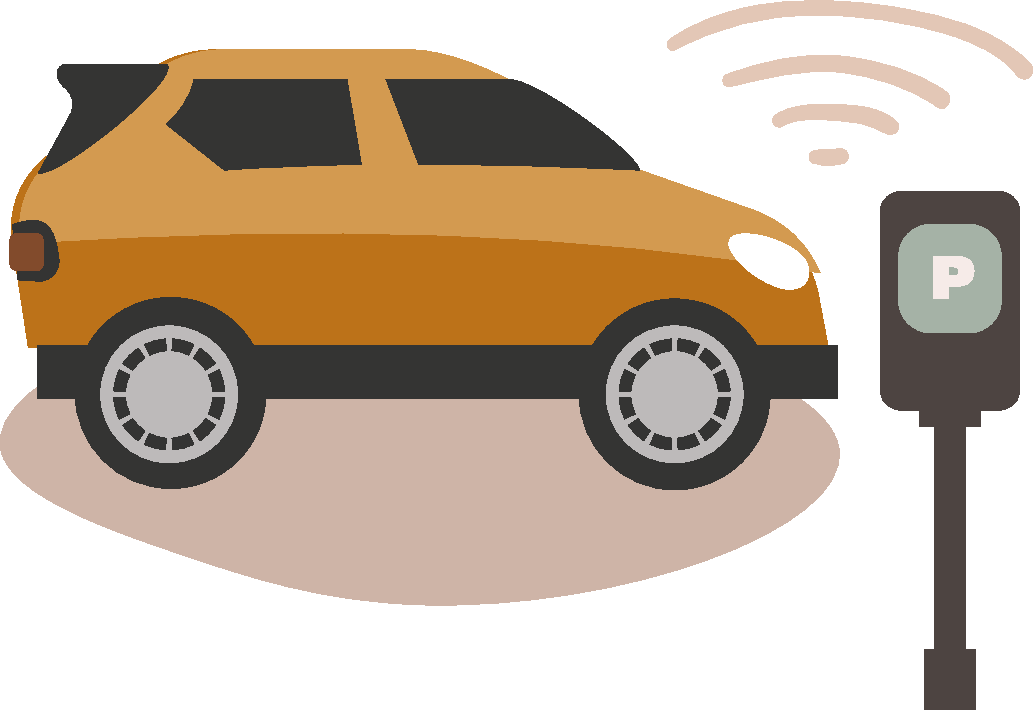
\includegraphics[keepaspectratio,alt={Fiscalização de estacionamento}]{img/am-park.pdf}}
\caption{Fiscalização de estacionamento}
\end{figure}

\end{tecnica}

Os serviços de fiscalização de estacionamento são um exemplo de como
algoritmos vêm sendo cada vez mais usados para automatizar serviços
públicos. Como algoritmos são exatos, rápidos e precisos, com frequência
promovem melhor eficiência, confiabilidade e consistência do serviço.
Paradoxalmente, algoritmos também podem cometer erros sistemáticos, ser
enviesados (\emph{bias}) e causar danos sérios. Sistemas de varredura,
por exemplo, podem apresentar mau funcionamento ou sofrer com falhas de
programação. Podem cometer enganos e sugerir que multas sejam emitidas
sem fundamento válido. Nesses casos, quem deve assumir a
responsabilidade --- e com base em quê?

Embora digamos coisas como ``sim, a culpa foi do algoritmo e ele é
responsável pela decisão errada'', não queremos dizer literalmente que
os algoritmos contemporâneos seriam moralmente culpados. Os algoritmos
são, antes, fatores causais que estão na base das decisões. Meras
causas, contudo, diferem de ações moralmente responsáveis.

Ainda que os próprios algoritmos não possam ser responsabilizados, por
não serem agentes morais ou jurídicos, as organizações que os projetam e
implantam podem ser consideradas moralmente responsáveis por meio de
estruturas de governança. Assim, no caso da cidade de Amsterdã, é o
fiscal humano que toma a decisão final --- e também assume a
responsabilidade. No entanto, um dia o fiscal humano também poderá ser
substituído por algoritmos. Quem, então, assumirá a responsabilidade?

\begin{tecnica}[Decisão automatizada vs. decisão autônoma]

\textbf{Sistemas automatizados} normalmente operam dentro de um conjunto
bem definido de parâmetros e são muito restritos quanto às tarefas que
podem executar. As decisões tomadas ou ações executadas por um sistema
automatizado baseiam-se em heurísticas ou regras predefinidas.

\textbf{Um sistema autônomo} aprende e se adapta a ambientes dinâmicos,
e evolui conforme o ambiente ao seu redor muda. Os dados com os quais
ele aprende e aos quais se adapta podem estar fora daquilo que foi
considerado quando o sistema foi implantado.

Automação ou autonomização são questões de grau e, portanto, formam um
contínuo, e não situações simples de sim ou não. Por exemplo, pode-se
dizer que um sistema é autônomo em relação ao controle humano até certo
grau.

\begin{figure}
\centering
\pandocbounded{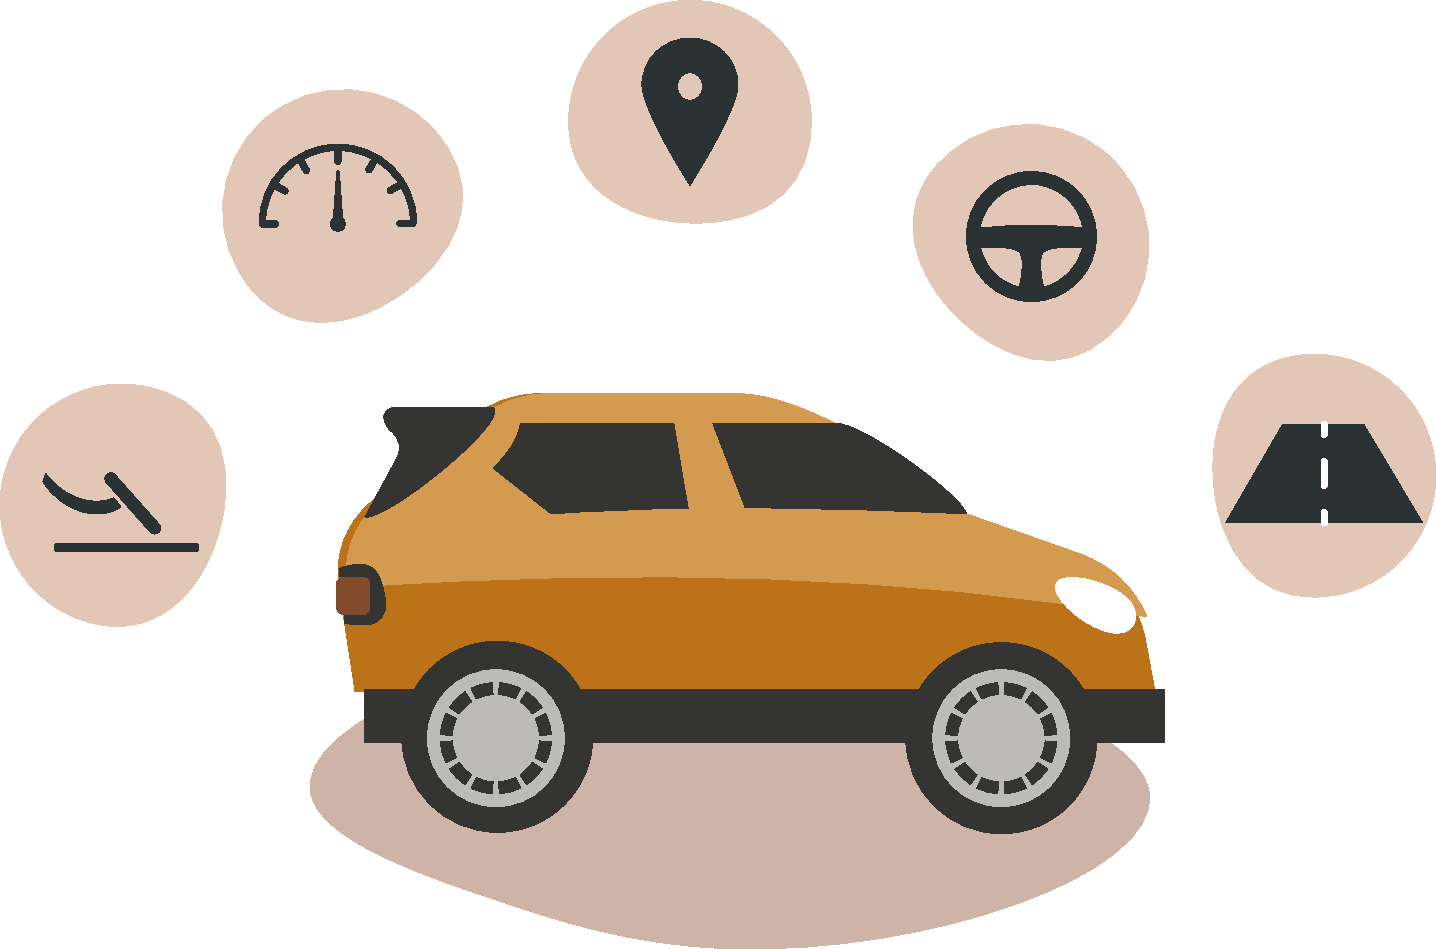
\includegraphics[keepaspectratio,alt={Níveis de automatização}]{img/levels-automatisation.pdf}}
\caption{Níveis de automatização}
\end{figure}

\end{tecnica}

\subsection{II. O que é
responsabilização?}\label{ii.-o-que-uxe9-responsabilizauxe7uxe3o}

Responsabilização (\emph{accountability}) significa o estado de ser
responsável ou de ter de prestar contas por um sistema, seu
comportamento e seus impactos potenciais. É o reconhecimento da
responsabilidade por ações, decisões e produtos.

A responsabilidade pode ser jurídica ou moral (ética).
\textbf{Juridicamente}, um ator é responsável por um evento quando um
sistema jurídico está apto a penalizá-lo por esse evento.
\textbf{Moralmente}, um ator é responsável por um ato se pode ser
culpado pela ação. Responsabilidade moral e jurídica são coisas
diferentes. Nem sempre coincidem: um agente pode ser juridicamente
responsável mesmo sem ser moralmente responsável, e vice-versa. Neste
curso, vamos nos concentrar apenas nos aspectos morais da
responsabilidade.

Na ética da IA, há três sentidos ou dimensões distintas de
responsabilização. Cada uma aponta para um meio de ação diferente:

\begin{itemize}
\tightlist
\item
  A questão de determinar a responsabilidade --- quais indivíduos (ou
  grupos) respondem pelo impacto dos algoritmos ou da IA? Quem é
  responsável por qual efeito dentro do sistema sociotécnico como um
  todo?
\item
  Uma característica do sistema social que desenvolve, produz e usa IA.
\item
  Uma característica do próprio sistema de IA.
\end{itemize}

\subsection{III. Quem deve ser culpado --- e por
quê?}\label{iii.-quem-deve-ser-culpado-e-por-quuxea}

\begin{figure}
\centering
\pandocbounded{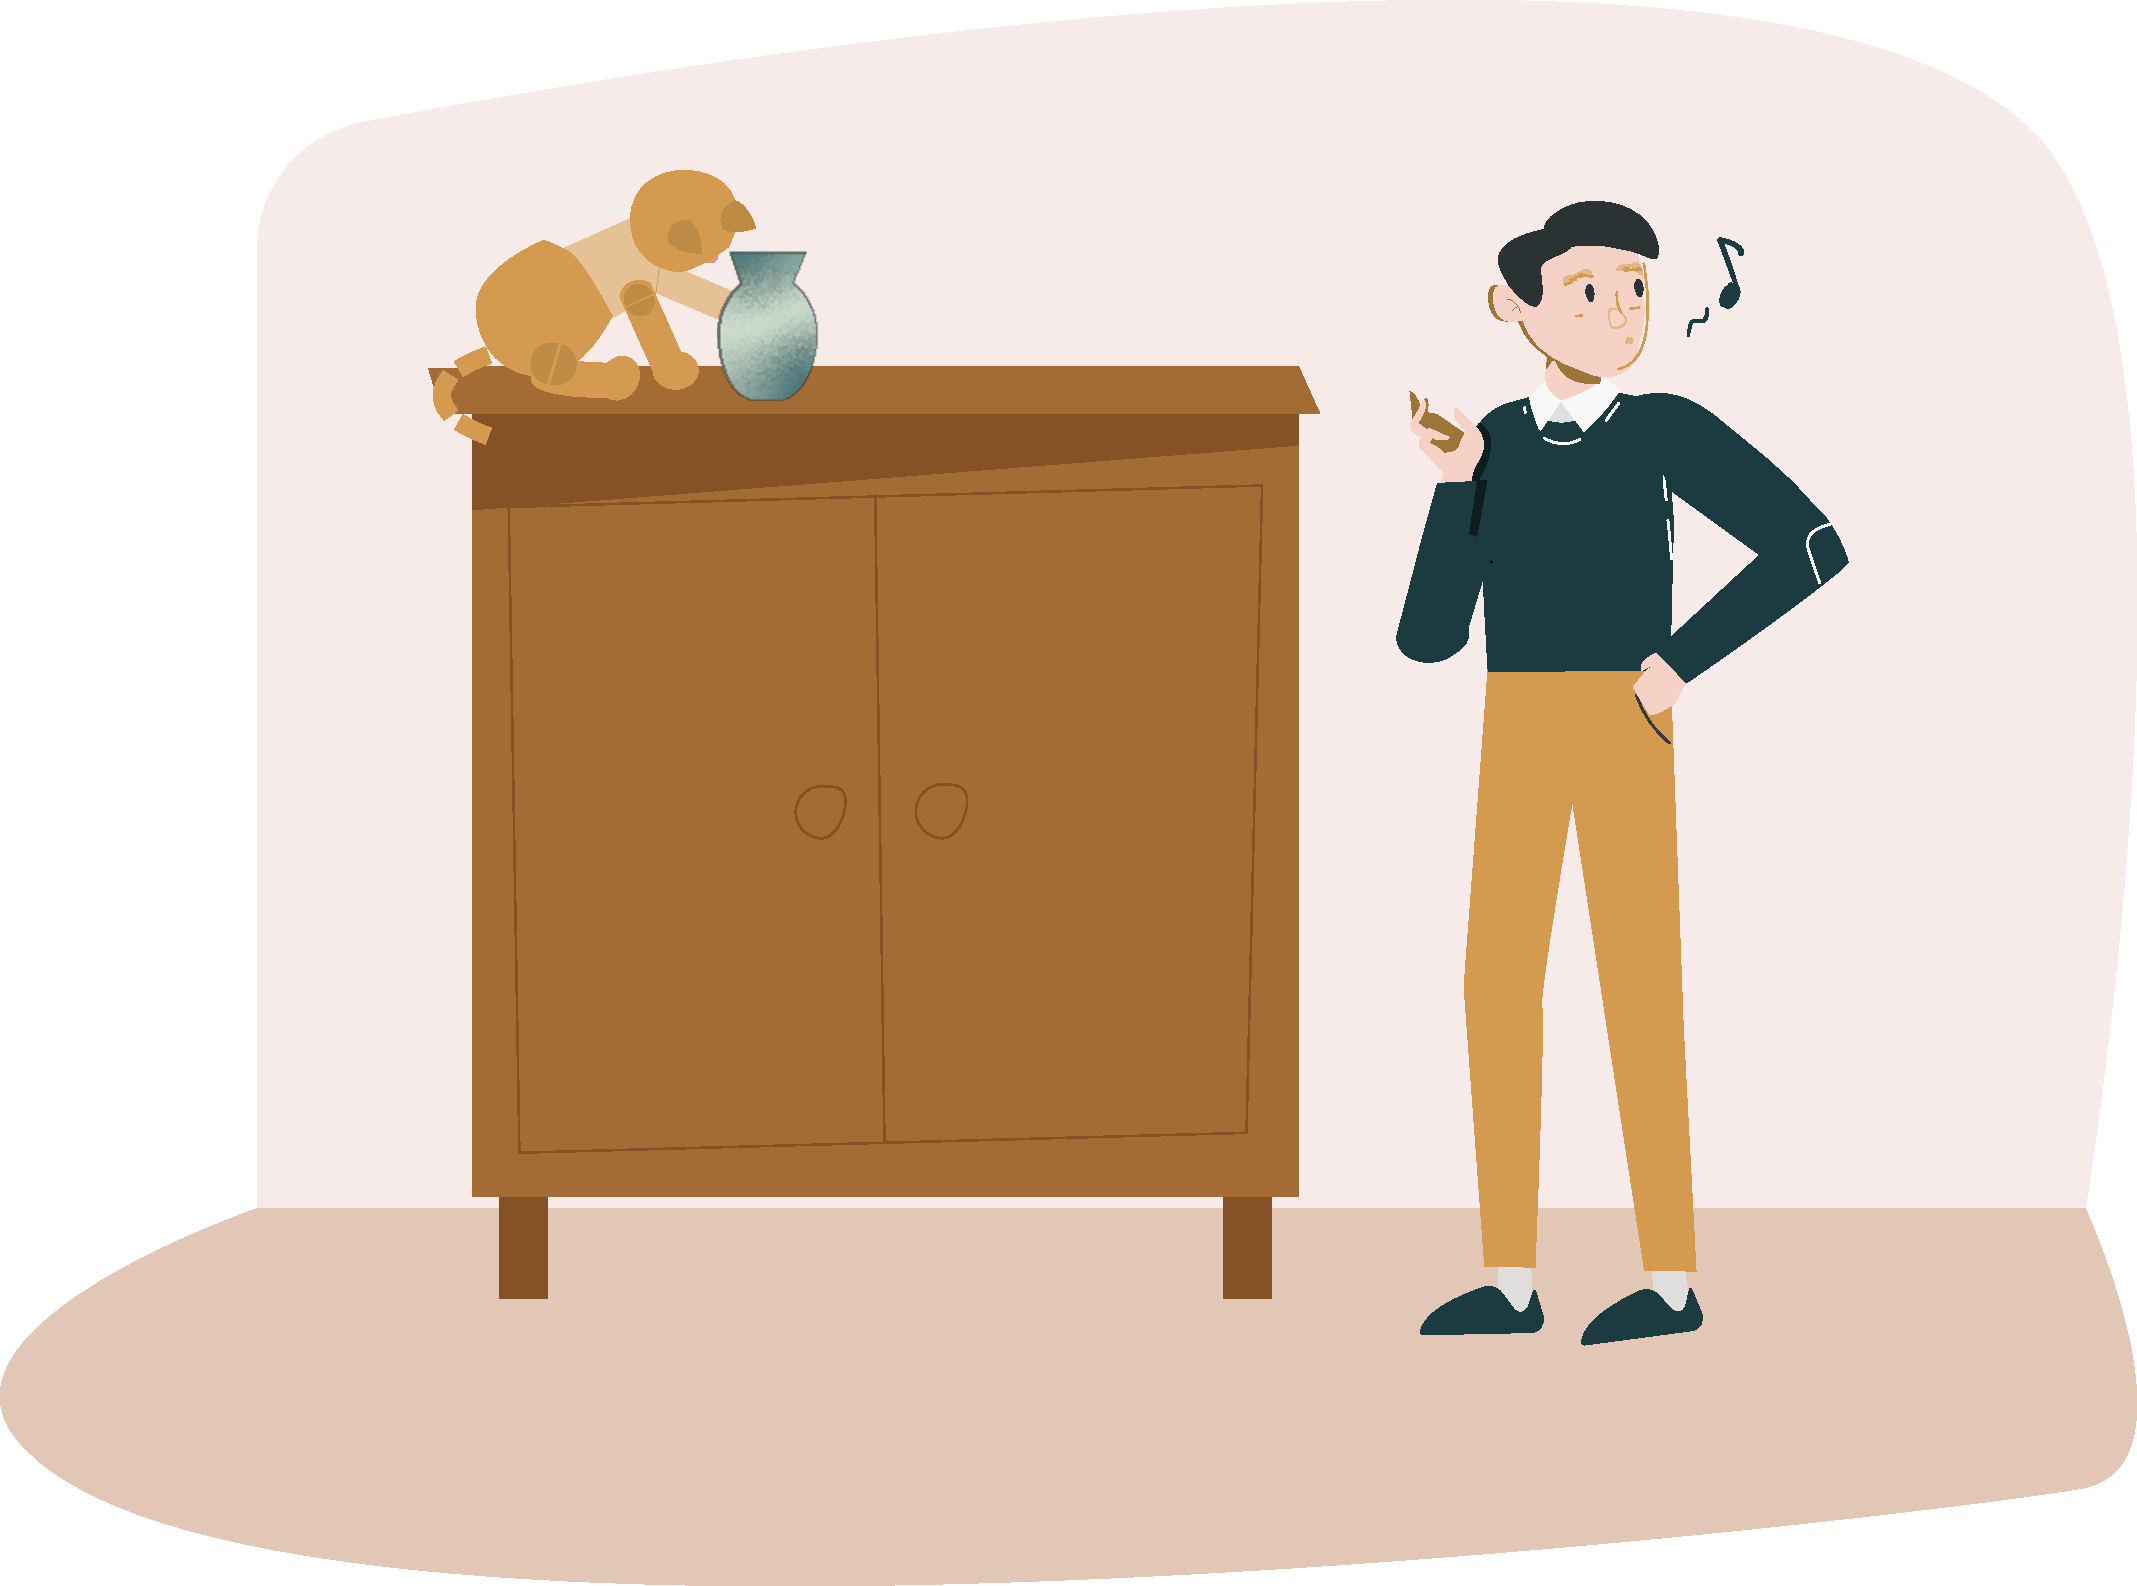
\includegraphics[keepaspectratio,alt={Agente e ação}]{img/agent-action.pdf}}
\caption{Agente e ação}
\end{figure}

Na ética, a responsabilização está estreitamente ligada ao conceito de
``agência moral''. Um agente moral é ``um agente capaz de agir com
referência ao certo e ao errado''. É importante notar que apenas agentes
morais são moralmente responsáveis por suas ações.

\textbf{Ações e omissões}

Filosoficamente, um agente moral é responsável primariamente por suas
próprias ações (``atos''). Às vezes, os agentes também são responsáveis
por não fazer algo, isto é, por ``omissões''. Assim, se eu mato alguém,
sou responsável por esse ato. Se apenas deixo alguém morrer, sou
responsável por não ter ajudado (omissão), ainda que eu não tenha matado
ativamente.

Omissões e ações não são moralmente equivalentes. É moralmente menos
grave omitir algo do que praticar um ato: é pior matar alguém ativamente
do que deixar essa pessoa morrer. Mas isso não torna as omissões
moralmente corretas. Ainda assim, não podemos ser responsáveis por todas
as coisas que deixamos de fazer. Somos responsáveis apenas por aquilo
que escolhemos fazer ou omitir de maneira deliberada e consciente.

\textbf{Autonomia}

Filosoficamente, a responsabilidade moral requer 1) autonomia moral e 2)
a capacidade de avaliar as consequências das ações. ``Autonomia moral''
significa a capacidade do agente de impor a si mesmo o código moral, de
modo autogovernado. Além disso, a autonomia requer:

\begin{itemize}
\tightlist
\item
  a capacidade de governar a si mesmo sem manipulação por outros e a
  possibilidade de agir sem constrangimentos externos ou internos;
\item
  a autenticidade dos desejos (valores, emoções etc.) que movem alguém a
  agir;
\item
  habilidades cognitivas suficientes --- ou seja, o agente deve ser
  capaz de avaliar, prever e comparar as consequências de suas ações e,
  também, de estimar os motivos que impulsionam a ação, usando critérios
  eticamente significativos.
\end{itemize}

\begin{filosofia}[Responsabilidade moral]

Immanuel Kant é um dos filósofos morais europeus mais célebres. Para
Kant, a razão prática --- nossa capacidade de usar razões para escolher
nossas próprias ações --- pressupõe que somos livres. As ações
baseiam-se em nossa própria vontade de utilizar uma lei moral para guiar
nossas decisões. Para Kant e para os kantianos, a tese é que essa
capacidade (a de impor a lei moral a nós mesmos) é a fonte última de
todo valor moral.

Assim, segundo Kant, devemos respeito moral a nós mesmos em virtude de
nossa autonomia. Mas devemos respeito semelhante a todas as outras
pessoas em virtude da capacidade delas. Portanto (pela segunda
formulação do célebre Imperativo Categórico de Kant), somos obrigados a
agir a partir de um respeito fundamental pelas outras pessoas em virtude
da autonomia delas. Desse modo, a autonomia serve tanto como modelo de
razão prática na determinação da obrigação moral quanto como a
característica das outras pessoas que as torna merecedoras de nosso
respeito moral. (Para uma discussão mais ampla, veja
\href{https://en.wikipedia.org/wiki/Categorical_imperative}{Immanuel
Kant e a filosofia moral}.)

\begin{figure}
\centering
\pandocbounded{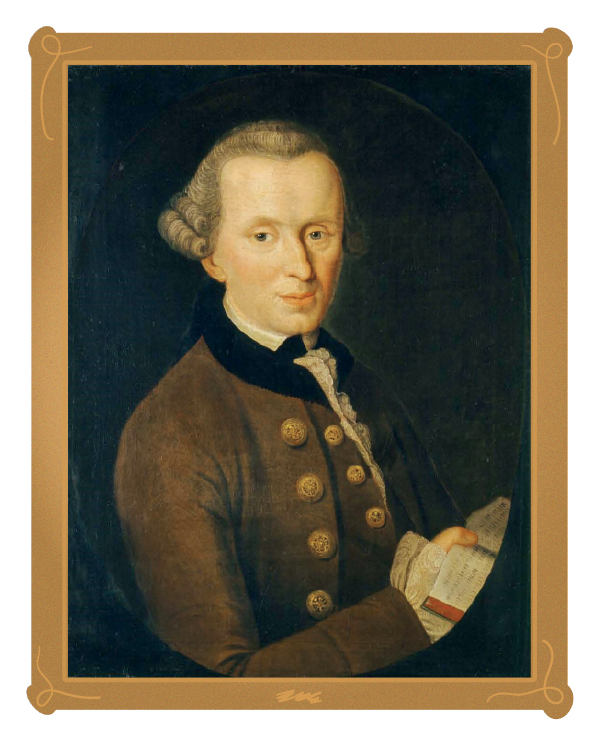
\includegraphics[keepaspectratio,alt={Retrato de Kant}]{img/kant.png}}
\caption{Retrato de Kant}
\end{figure}

\end{filosofia}

\begin{reflexao}[Exercícios desta seção]

O material original traz aqui um questionário interativo. As perguntas
não constam do repositório de origem --- ficam no banco de dados da
plataforma. O exercício correspondente deve ser redigido em
\texttt{exercicios/capitulo03-exercicios.md}.

\end{reflexao}

\subsection{IV. O problema de individualizar
responsabilidades}\label{iv.-o-problema-de-individualizar-responsabilidades}

A responsabilização é frequentemente entendida como uma obrigação
jurídica e ética de um indivíduo ou organização de aceitar a
responsabilidade pelo uso de sistemas de IA e de divulgar os resultados
de maneira transparente. Essa formulação pressupõe uma ``relação de
poder''. Ela individualiza quem está no controle e quem deve ser
culpado.

Contudo, tem se mostrado notoriamente difícil estabelecer critérios
específicos sobre como, exatamente, as responsabilidades devem ser
individualizadas, direcionadas e definidas. Em muitos países há debates
em curso sobre essas questões. Atores internacionais, como a União
Europeia e o G7, as trataram como desafios em aberto.

Por que é tão difícil estabelecer critérios sobre quem é responsável?

\begin{itemize}
\item
  \textbf{Primeiro}, a qualidade das responsabilidades difere. Um ator é
  responsável por uma ação ou omissão específica, mas a qualidade da
  responsabilidade depende da parte envolvida. Assim, embora ao escolher
  uma ação você possa assumir a responsabilidade, a qualidade dessa
  responsabilidade depende também de suas propriedades. As tecnologias
  inteligentes complicam ainda mais esse quadro.

  À medida que delegamos cada vez mais tarefas e funções de tomada de
  decisão a algoritmos, também moldamos as estruturas de decisão. A IA
  amplia nossa inteligência ao nos dar mais poder computacional,
  permitir melhores previsões e aprimorar nosso aparato sensorial.
  Humanos e máquinas tornam-se híbridos cognitivos. Cooperam
  cognitivamente (pensamento) e epistemicamente (conhecimento), tanto no
  nível individual quanto no coletivo. Isso cria propriedades
  sistêmicas.

  Costuma-se pensar que basta um humano permanecer ``no circuito''
  (\emph{in-the-loop}) ou ``sobre o circuito'' (\emph{on-the-loop}) ---
  ou seja, que em algum ponto da tomada de decisão um indivíduo humano
  seria capaz de monitorar o sistema artificial ou nele intervir. No
  entanto, à medida que algoritmos entram na tomada de decisão, digamos,
  na governança do setor público, a decisão coletiva pode assumir uma
  forma muito complexa e altamente distribuída. Individualizar e
  endereçar os fatores de modo a garantir que um humano permaneça no
  circuito pode ser realmente difícil.
\item
  \textbf{Segundo}, a tecnologia também pode assumir uma forma
  persuasiva: ela influencia e controla as pessoas. Um exemplo clássico
  é o som do alarme do cinto de segurança. Em muitos carros, se os
  cintos não estiverem afivelados, um bipe constante é acionado. Isso
  pode ser entendido como uma forma de influência controladora --- nesse
  caso, uma espécie de coerção. O motorista só consegue interromper o
  som afivelando o cinto. Aplicações algorítmicas contemporâneas podem
  ter cada vez mais características desse tipo: elas propõem, sugerem e
  limitam as opções.

  Mas uma ação só é praticada voluntariamente se for praticada
  intencionalmente (quem age está ``no controle'') e estiver livre de
  influências controladoras. O motorista está livre de influências
  controladoras se o sistema do cinto de segurança o força a reagir ao
  bipe? Ou: estamos livres de controle se os algoritmos decidem as fotos
  de quem veremos nos sites de relacionamento, ou que música estamos
  prestes a ouvir? Qual é, exatamente, a diferença entre sugestão
  algorítmica, controle e manipulação?

  Naturalmente, a tecnologia persuasiva deveria cumprir a exigência de
  voluntariedade para garantir a autonomia. Os algoritmos complicam essa
  questão, uma vez que a voluntariedade pressupõe uma compreensão
  suficiente do uso daquela tecnologia específica. Mas o que significa
  ``compreender'', e qual é, de fato, o grau suficiente? Qual é a
  leitura correta de ``compreensibilidade'' --- ``transparência'',
  ``explicabilidade'' ou ``auditabilidade''? Quanto, e o que exatamente,
  um usuário deveria entender sobre a tecnologia? Quando alguém pode
  genuinamente avaliar se quer ou não usar aquela tecnologia em
  particular? Examinaremos esse tema em mais detalhe no capítulo 4.
\end{itemize}

\begin{reflexao}[Exercícios desta seção]

O material original traz aqui um questionário interativo. As perguntas
não constam do repositório de origem. O exercício correspondente deve
ser redigido em \texttt{exercicios/capitulo03-exercicios.md}.

\end{reflexao}

\subsubsection{Estudo de caso: o diretor digital de
Helsinque}\label{estudo-de-caso-o-diretor-digital-de-helsinque}

\begin{figure}
\centering
\pandocbounded{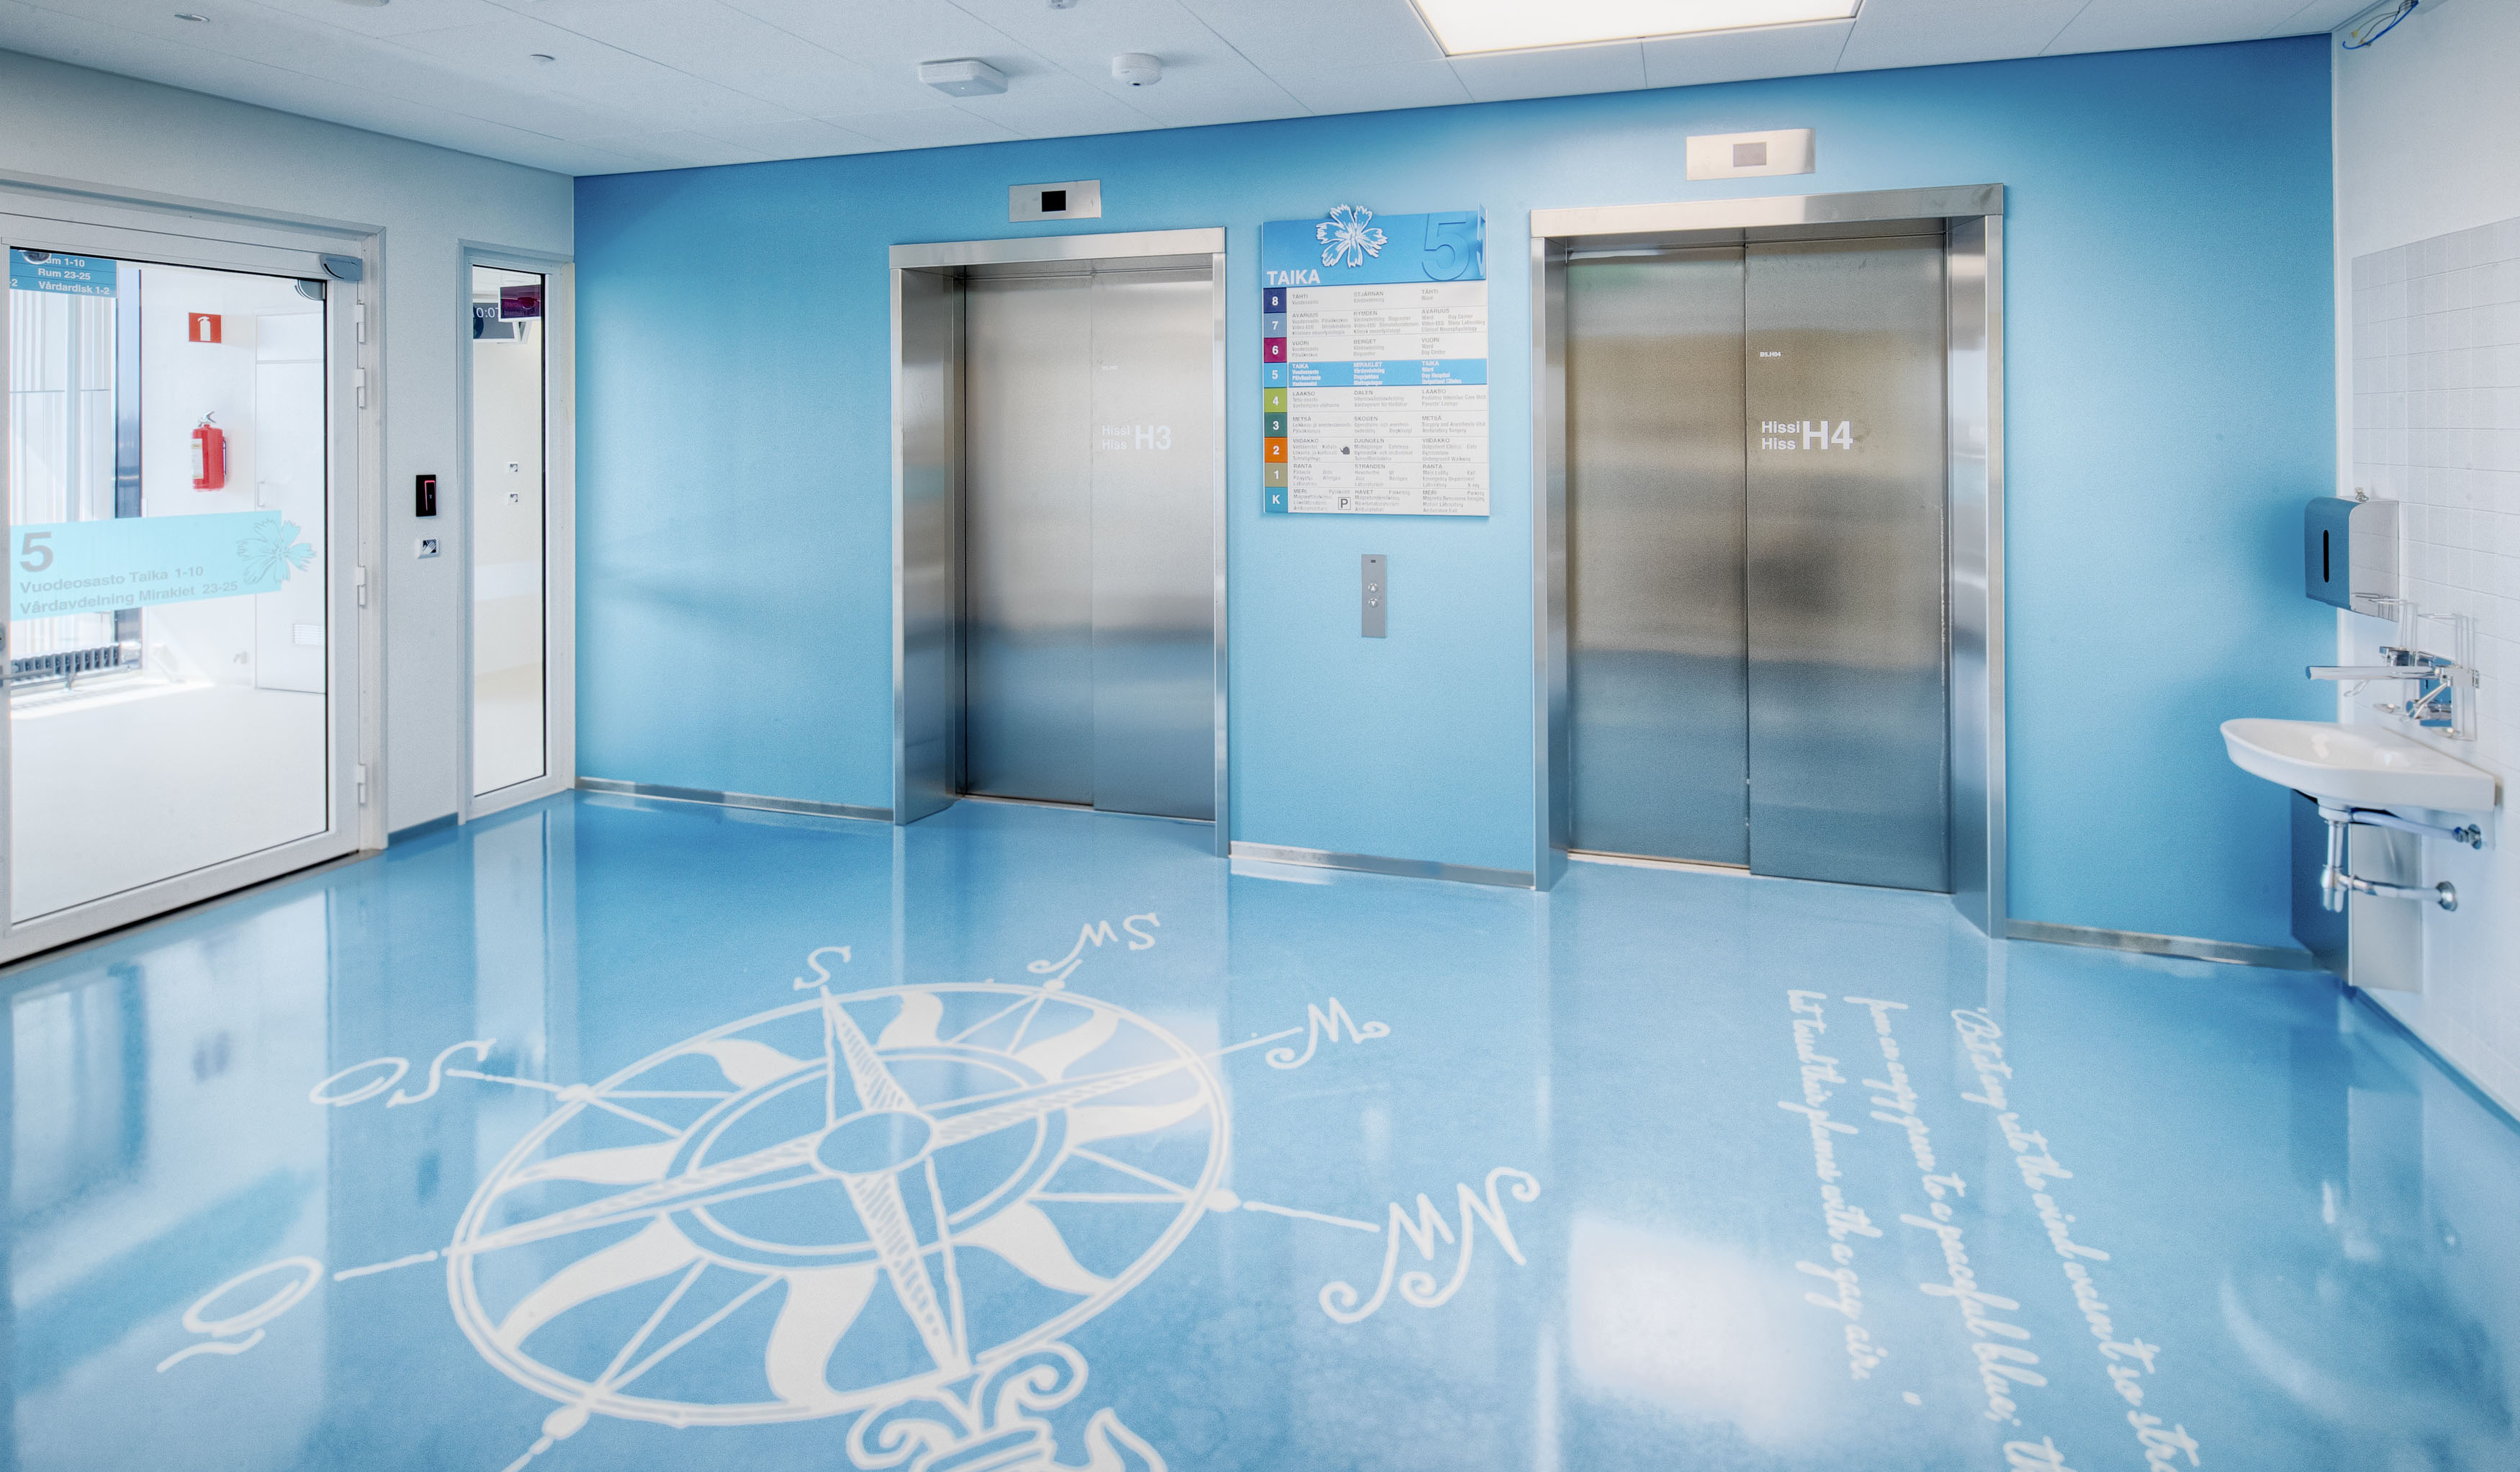
\includegraphics[keepaspectratio,alt={Hospital}]{img/_MS_9489_HDR_cropped.jpg}}
\caption{Hospital}
\end{figure}

\emph{Imagem © Cidade de Helsinque / Comunicação}

\begin{caso}[De quem é a responsabilidade?]

Voltemos ao caso da saúde em Helsinque (mencionado no início do capítulo
2). Suponha que você seja o diretor digital da cidade de Helsinque.
Pedem que você avalie se a organização de saúde da cidade deveria migrar
de uma saúde reativa para uma saúde preventiva. Você lê um relatório que
discute métodos novos, baseados em aprendizado de máquina (\emph{machine
learning}), que ajudariam as autoridades de saúde a prever os possíveis
riscos de saúde dos cidadãos.

O relatório menciona muitas vantagens, como prevenção de doenças, melhor
estimativa de impacto e melhor planejamento dos serviços básicos de
saúde. Contudo, também revela algumas preocupações com privacidade,
polarização e a possível ameaça de discriminação não intencional. Além
disso, o relatório levanta a questão fundamental do papel da cidade. Se
a cidade tem informação sobre os riscos potenciais de saúde e não age
sobre esses dados, a cidade é moralmente responsável por negligência?

O relatório também aborda a questão de individualizar responsabilidades.
Se o sistema fosse aplicado na prática, haveria sempre o risco de que
cometesse um erro. Quem devemos culpar se isso acontecer?

\end{caso}

\begin{reflexao}[Exercícios desta seção]

No material original, este estudo de caso termina com uma tarefa
dissertativa sobre a responsabilidade de um diretor digital, avaliada
por revisão por pares. Redija a versão em português desse exercício em
\texttt{exercicios/capitulo03-exercicios.md}.

\end{reflexao}

\subsection{Referências}\label{referuxeancias}

Kant, I. (1785). \emph{Grundlegung zur Metaphysik der Sitten}
{[}Fundamentação da Metafísica dos Costumes{]}.

Cidade de Amsterdã --- sistema automatizado de fiscalização de
estacionamento.

\begin{center}\rule{0.5\linewidth}{0.5pt}\end{center}

\begin{licenca}

\textbf{Material original:} \emph{Ethics of AI}, um curso online
gratuito da Universidade de Helsinque. Professores responsáveis:
Anna-Mari Rusanen e Jukka K. Nurminen. Demais contribuintes principais:
Santeri Räisänen, Sasu Tarkoma e Saara Halmetoja. Disponível em
\url{https://ethics-of-ai.mooc.fi/}.

\textbf{Esta versão:} tradução e adaptação para o português brasileiro
realizada por José Lucas Lira Bizil, Fernando Mazzeto Lisboa Lima e
Matheus da Silva Fernandes, no âmbito do Programa CiberExt 26-29
(FEELT38103), Universidade Federal de Uberlândia, 2026. Esta é uma obra
derivada; os autores originais não a revisaram nem a endossam.

\textbf{Licença:} Creative Commons
Atribuição-NãoComercial-CompartilhaIgual 4.0 Internacional (CC BY-NC-SA
4.0) ---
\url{https://creativecommons.org/licenses/by-nc-sa/4.0/deed.pt-br}.

\end{licenca}

\end{document}
